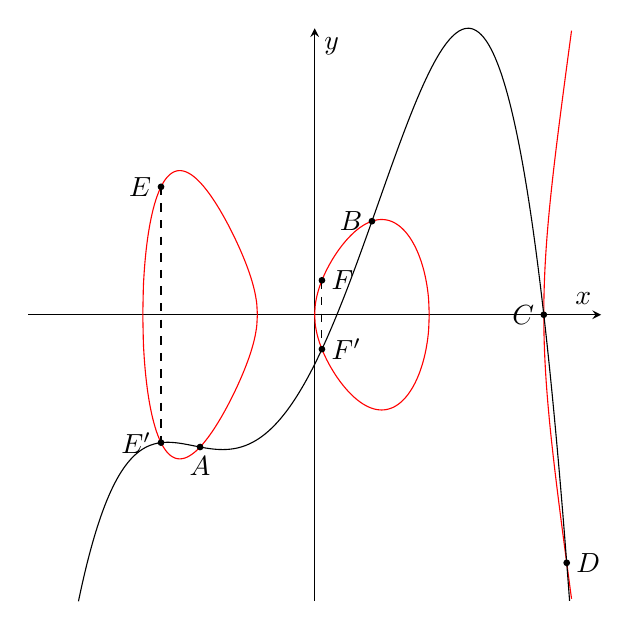
\begin{tikzpicture}
\pgfplotsset{ticks=none}
\begin{axis}[
        xmin=-5,xmax=5,
        ymin=-15,ymax=15,
        unit vector ratio={3 1},
        xlabel={$x$},
        ylabel={$y$},
        scale only axis, axis lines=middle,
        domain=-2.279018:3,
        samples=201,smooth,clip=false,
    ]
\addplot[red, domain=-3:-1] {sqrt(x^5-2*x^4-13*x^3+14*x^2+24*x)};
\addplot[red, domain=-3:-1] {-sqrt(x^5-2*x^4-13*x^3+14*x^2+24*x)};
\addplot[red, domain=0:2] {sqrt(x^5-2*x^4-13*x^3+14*x^2+24*x)};
\addplot[red, domain=0:2] {-sqrt(x^5-2*x^4-13*x^3+14*x^2+24*x)};
\addplot[red, domain=4:4.484] {sqrt(x^5-2*x^4-13*x^3+14*x^2+24*x)};
\addplot[red, domain=4:4.484] {-sqrt(x^5-2*x^4-13*x^3+14*x^2+24*x)};
\addplot[black, domain=-4.123:4.45] {-0.135479279399*x^4-0.269857841745*x^3+1.91253148281*x^2+5.98710284966*x-2.59531772575};
\draw[fill=black] (-2, -6.92820323028) circle (1pt);
\draw[fill=black] (-2, -6.92820323028) node[below] {$A$};
\draw[fill=black] (1, 4.89897948557) circle (1pt);
\draw[fill=black] (1, 4.89897948557) node[left] {$B$};
\draw[fill=black] (4, 0) circle (1pt);
\draw[fill=black] (4, 0) node[left] {$C$};
\draw[fill=black] (4.4, -12.9919605911) circle (1pt);
\draw[fill=black] (4.4, -12.9919605911) node[right] {$D$};
\draw[fill=black] (-2.682, -6.699) circle (1pt);
\draw[fill=black] (-2.682, -6.699) node[left] {$E'$};
\draw[fill=black] (0.127,-1.803) circle (1pt);
\draw[fill=black] (0.127,-1.803) node[right] {$F'$};
\draw[fill=black] (-2.682, 6.699) circle (1pt);
\draw[fill=black] (-2.682, 6.699) node[left] {$E$};
\draw[fill=black] (0.127,1.803) circle (1pt);
\draw[fill=black] (0.127,1.803) node[right] {$F$};
\draw[dashed] (0.127,1.803) -- (0.127,-1.803);
\draw[dashed] (-2.682, 6.699) -- (-2.682, -6.699);
\end{axis}
\end{tikzpicture}